% !TeX encoding = UTF-8
% !TeX program = xelatex
% !TeX spellcheck = en_US

\documentclass[degree=project,degree-type=project,cjk-font=noto]{thuthesis}
\usepackage{mathtools}
\usepackage{tikz}
\usetikzlibrary{shapes,arrows}
\usepackage[autosize]{dot2texi}
% Syntax Highlighting in LaTeX, need pygments
% Must build with xelatex -shell-escape -enable-8bit-chars.
\usepackage{minted}
% https://tex.stackexchange.com/a/112573
\usepackage{tcolorbox}
\usepackage{etoolbox}
\BeforeBeginEnvironment{minted}{\begin{tcolorbox}}%
\AfterEndEnvironment{minted}{\end{tcolorbox}}%
% color for minted
\definecolor{friendlybg}{HTML}{f0f0f0}


% 论文基本配置,加载宏包等全局配置
\thusetup{
    output = electronic,
    title  = {作业二},
    author  = {肖文韬},
    studentid = {2020214245},
    major = {电子信息(计算机技术)},
    email = {xwt20@mails.tsinghua.edu.cn},
    course = {密码学与网络安全},
    include-spine = false,
}


\usepackage{float}
\usepackage[sort]{natbib}
\bibliographystyle{thuthesis-numeric}
\graphicspath{{figures/}}


\setlist[enumerate,1]{label=\arabic*.}
\setlist[enumerate,2]{label=(\alph*)}
\setlist[enumerate,3]{label=\roman*.}
\setlist[enumerate,4]{label=\greek*}


\begin{document}

% 封面
\maketitle

\frontmatter
% % !TeX root = ../thuthesis-example.tex

% 中英文摘要和关键字

\begin{abstract}
  论文的摘要是对论文研究内容和成果的高度概括。摘要应对论文所研究的问题及其研究目
  的进行描述,对研究方法和过程进行简单介绍,对研究成果和所得结论进行概括。摘要应
  具有独立性和自明性,其内容应包含与论文全文同等量的主要信息。使读者即使不阅读全
  文,通过摘要就能了解论文的总体内容和主要成果。

  论文摘要的书写应力求精确、简明。切忌写成对论文书写内容进行提要的形式,尤其要避
  免“第 1 章……;第 2 章……;……”这种或类似的陈述方式。

  本文介绍清华大学论文模板 \thuthesis{} 的使用方法。本模板符合学校的本科、硕士、
  博士论文格式要求。

  本文的创新点主要有:
  \begin{itemize}
    \item 用例子来解释模板的使用方法;
    \item 用废话来填充无关紧要的部分;
    \item 一边学习摸索一边编写新代码。
  \end{itemize}

  关键词是为了文献标引工作、用以表示全文主要内容信息的单词或术语。关键词不超过 5
  个,每个关键词中间用分号分隔。(模板作者注:关键词分隔符不用考虑,模板会自动处
  理。英文关键词同理。)

  % 关键词用“英文逗号”分隔
  \thusetup{
    keywords = {TeX, LaTeX, CJK, 模板, 论文},
  }
\end{abstract}

\begin{abstract*}
  An abstract of a dissertation is a summary and extraction of research work
  and contributions. Included in an abstract should be description of research
  topic and research objective, brief introduction to methodology and research
  process, and summarization of conclusion and contributions of the
  research. An abstract should be characterized by independence and clarity and
  carry identical information with the dissertation. It should be such that the
  general idea and major contributions of the dissertation are conveyed without
  reading the dissertation.

  An abstract should be concise and to the point. It is a misunderstanding to
  make an abstract an outline of the dissertation and words ``the first
  chapter'', ``the second chapter'' and the like should be avoided in the
  abstract.

  Key words are terms used in a dissertation for indexing, reflecting core
  information of the dissertation. An abstract may contain a maximum of 5 key
  words, with semi-colons used in between to separate one another.

  \thusetup{
    keywords* = {TeX, LaTeX, CJK, template, thesis},
  }
\end{abstract*}


% 目录
% \tableofcontents

% 插图和附表清单
% \listoffiguresandtables
% \listoffigures           % 插图清单

% 正文部分
\mainmatter

\chapter{作业内容}

\begin{enumerate}
  \setlength{\itemsep}{3\parskip}
  \item 考虑一个密码体系 $M = \{a, b, c\}, K = \{k_1, k_2, k_3\}$ 和 $C = \{1, 2, 3, 4\}$, 将明文 M 使用密钥 K 加密为密文 C。假设加密矩阵如下表。
  \begin{table}[htp]
  	\centering
  	\begin{tabular}{|c|c|c|c|}
  		\hline
  		& a & b & c \\\hline
  		$k_1$ & 2 & 3 & 4 \\\hline
  		$k_2$ & 3 & 4 & 1 \\\hline
  		$k_3$ & 1 & 2 & 3 \\\hline
	\end{tabular}
  \end{table}
  \newline
  已知密钥概率分布 $p(k_3) = 1/2, p(k_2) = p(k_1) = 1/4$, 且明文概率分布 $p(a) = 1/3, p(b) = 8/15, p(c)  = 2/15$。请计算 $H(M), H(K), H(C), H(M|C), H(K|C)$。
  \newline
  {\heiti 解:}
  \begin{align}
  	H(M) &= \sum_i p(M_i) I(M_i) = -\sum_i p(M_i) \log p(M_i) \approx 1.3996 \\
  	H(K) &\approx 1.5 \\
  	H(C) &\approx 1.9408 \quad (p(C) = [0.2, 0.35, 0.2833, 0.1667]) \\
  	H(M|C) &= H(MC) - H(C) \nonumber \\
          &= -\sum_i \sum_j p(M_i, C_j) \log p(M_i, C_j) \approx 2.8996 \\
  	H(K|C) &= H(KC) - H(C) \approx 2.8996
  \end{align}

\item 计算英文字母的凯撒密码的唯一解距离。
\newline
{\heiti 解:}
\newline
\begin{equation}
N = \frac{H(K)}{D} = - \frac{\log\left(\frac{1}{26}\right)}{3.2} \approx 2
\end{equation}
\newline

\item 计算重复周期为 6 的维吉尼亚密码的唯一解距离。
\newline
{\heiti 解:}
\newline
\begin{equation}
N = \frac{H(K)}{D} = - \frac{\log \left(\frac{1}{26^6}\right)}{3.2} \approx 9
\end{equation}
\newline

\item 某次 AES 加密的轮函数过程中,字节替代的结果为:
\begin{equation}
  A = \begin{bmatrix}
  87 & F2 & 4D & 97 \\
  EC & 6E & 4C & 90 \\
  4A & C3 & 46 & E7 \\
  8C & D8 & 95 & A6
  \end{bmatrix}
\end{equation}
{\heiti 解:}
\newline
求这个矩阵经过行移位变换后的结果,以及经过列混淆后第三行第一列的值。

\begin{figure}[!htp]
\centering%
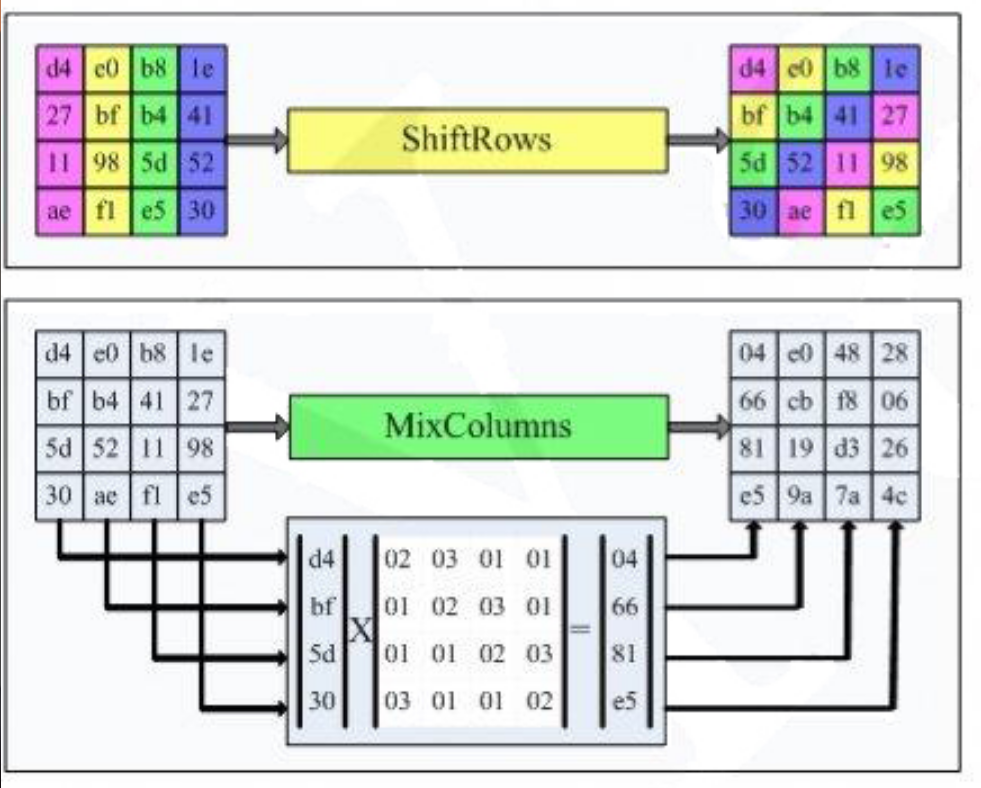
\includegraphics[width=.7\linewidth]{aes.png}
  \caption{移位变换和列混淆的具体过程}
  \label{fig:aes}
\end{figure}

移位变换和列混淆的具体过程如图~\ref{fig:aes}所示。
移位表换后的结果为 $B$.

\begin{equation}
  B = \begin{bmatrix}
  87 & F2 & 4D & 97 \\
  6E & 4C & 90 & EC \\
  46 & E7 & 4A & C3 \\
  A6 & 8C & D8 & 95
  \end{bmatrix}
\end{equation}

列混淆后的结果为 $C$.

\begin{equation}
  C = \begin{bmatrix}
  47 & 40 & A3 & 4C \\
  37 & D4 & 70 & 9F \\
  94 & E4 & 3A & 42 \\
  ED & A5 & A6 & BC
  \end{bmatrix}
\end{equation}

\item 思考题:为何 AES 加密算法的最后一轮与前 9 轮不同?

{\heiti 解:}
\newline
AES算法在处理的轮数上只有最后一轮与前面 9 轮不同之处在于最后一轮少了列混淆处理。
理由:
\newline\newline
在正常的 AES 轮中,列混淆会在轮密钥加操作之前进行。
不过,也可以调换这些操作的顺序。先执行轮密钥加操作,再执行列混淆操作,稍加修改,就可以收到同样的结果。
因此,可以认为最后的列混淆不会增加任何安全性,因为它是一个不加键、可逆的操作,可以使其成为最后一轮的最后一步。
\newline\newline
然而理论上我们可以进行攻击。考虑到一个AES变体,其中列混淆在最后一轮加密中执行。
为了攻击解密函数,攻击者可能会交换列混淆和轮密钥加的顺序,这样他就可以直接撤销列混淆。
现在假设他能够(以某种方式)恢复轮密钥加中使用的轮密钥的一些信息。
因为他交换了操作,所以他恢复的实际上并不是键表(Key schedule)吐出的轮密钥的信息,而是应用了逆列混淆的轮密钥的信息。
\end{enumerate}

\end{document}
